\chapter{Zero-Knowledge Proofs for LWE}

\section{Introduction}

LWE (Learning with error) problem is one of the fundamental lattice problem upon which lots of the lattice-based cryptography rests. LWE states that for a tuple $(A, u)$ it is hard to find a small $s$ and a small $e$ such that $u = As+e$. In this chapter, we explore a protocol in \cite{lwe} that makes use of polynomials to prove knowledge of $s$ and $e$ with small elements that satisfy:
$$
    As + e = u
$$

\begin{definition}[Relation $R_{LWE}$]
The relation $R_{LWE}$ is the sets of tuples
$$
    (\mathbb{X}, \mathbb{W}) = ((\mathbb{F}, n, m, A, u), (s, e))
$$ 
such that $A \in \mathbb{F}^{n \times m}$, $u \in \mathbb{F}^{n}$, $s \in \{-1, 0, 1\}^{m}$, $e \in \{-1, 0, 1\}^{n}$ and $As + e = u$.
\end{definition}

% \section{LWE Protocol}

% In this protocol, the prover $\mathcal{P}$ is allowed to send a tuple $a = (a_1, \cdots, a_l)$ where $a_i \in \mathbb{F}^k$. And the verifier $\mathcal{V}$ has linear query access to it by send a coefficient tuple $b = (b_1, \cdots, b_l)$ where $b_i \in \mathbb{F}$. The response will a array $e$ where $e_j = \langle (a_1[j], \cdots, a_l[j]), b  \rangle$.

% \subsection{Formal Description}

% Prover $\mathcal{P}$'s input: $A \in \mathbb{F}^{n \times m}$, $u \in \mathbb{F}^{n}$, $s \in \{-1, 0, 1\}^{m}$ and $e \in \{-1, 0, 1\}^{n}$ such that $u = As + e$.

% Verifier $\mathcal{V}$'s input: $A \in \mathbb{F}^{n \times m}$, $u \in \mathbb{F}^{n}$.

% The protocol proceeds as follows.



% \begin{itemize}
%     \item $\mathcal{P}$ samples $t \leftarrow \mathbb{F}^{m}$ and computes the polynomials $f(X)=tX+s$ and $d(X)=u-Af(X)$.
%     \item $\mathcal{P}$ computes the polynomials:
% \begin{equation}
% \label{eq:lwe1}
%     \frac{1}{X} f(X) \circ [f(X) - 1^m] \circ [f(X) + 1^m] = v_2X^2 + v_1X + v_0
% \end{equation}
% \begin{equation}
% \label{eq:lwe2}
%     \frac{1}{X} d(X) \circ [d(X) - 1^n] \circ [d(X) + 1^n] = w_2X^2 + w_1X + w_0
% \end{equation}

%     \item $\mathcal{P}$ sends $(f_1, f_0), (d_1, d_0), (v_2, v_1, v_0), (w_2, w_1, w_0)$ to $\mathcal{V}$, and $\mathcal{V}$ has linear query access to each of these tuples. If the prover is honest, $(f_1, f_0)$ should equal to $(t, s)$ and $(d_1, d_0)$ should equal to $(-At, u-As)$.
    
%     \item $\mathcal{V}$ sample a random challenge $x \leftarrow \mathbb{F}^*$.
    
%     \item $\mathcal{V}$ sends linear query to $(f_1, f_0)$ with coefficient vector $(x, 1)$. Denote the response as $f \in \mathbb{F}^m$.
%     \item $\mathcal{V}$ sends linear query to $(d_1, d_0)$ with coefficient vector $(x, 1)$. Denote the response as $d \in \mathbb{F}^n$.
%     \item $\mathcal{V}$ sends linear query to $(v_2, v_1, v_0)$ with coefficient vector $(x^2, x, 1)$. Denote the response as $g \in \mathbb{F}^m$.
%     \item $\mathcal{V}$ sends linear query to $(w_2, w_1, w_0)$ with coefficient vector $(x^2, x, 1)$. Denote the response as $h \in \mathbb{F}^n$.
    
%     \item $\mathcal{V}$ will check whether the following equation holds:
% $$
%     g \overset{?}{=} \frac{1}{x} (f \circ [f - 1^m] \circ [f + 1^m])
% $$
% $$
%     h \overset{?}{=} \frac{1}{x} (d \circ [d - 1^n] \circ [d + 1^n])
% $$
% \end{itemize}

% \begin{lemma}
% \label{lemma:lwepc}

% LWE = ($\mathcal{P}$, $\mathcal{V}$) has \textbf{perfect completeness}.

% \end{lemma}
% \begin{proof}

% According to equation \ref{eq:lwe1}, the first checking will succeed. And according to equation \ref{eq:lwe2}, the second checking will succeed.

% \end{proof}

% \begin{lemma}
% \label{lemma:lwese}

% LWE = ($\mathcal{P}$, $\mathcal{V}$) has has soundness error at most $\frac{2}{q}$, where $q$ is the size of the underlying field.

% \end{lemma}
% \begin{proof}

% Suppose $(\mathbb{X}, \mathbb{W}) = ((\mathbb{F}, n, m), (A, u, s, e))$ is not in relation $R_{LWE}$. 
% Then at least at one position $i$, either $\frac{1}{X} f_i(X)[f_i(X) - 1][f_i(X) + 1]$ and $v_{2, i}X^2 + v_{1, i}X + v_{0, i}$ are different polynomials, or $\frac{1}{X} d_i(X)[d_i(X) - 1][d_i(X) + 1]$ and $w_{2, i}X^2 + w_{1, i}X + w_{0, i}$ are different polynomials. Note that they are polynomials with degree equal 2. According to Schwartz-Zippel lemma, they can agree on at most 2 evaluation points. Since challenge $x$ is sampled randomly from $\mathbb{F}$, the probability this event appears is at most $\frac{2}{q}$.

% Suppose $(\mathbb{X}, \mathbb{W}) = ((\mathbb{F}, n, m), (A, u, s, e))$ is in relation $R_{LWE}$, but the prover $\mathbb{P}$ sends a incorrect polynomials $g^\prime$ or $h^\prime$. Likewise, since they are polynomials with degree equal 2, according to Schwartz-Zippel lemma, they can agree on at most 2 evaluation points. The probability that the verifier accepts the protocol is also at most $\frac{2}{q}$.


% \end{proof}

% \begin{lemma}
% \label{lemma:lwezk}

% LWE = ($\mathcal{P}$, $\mathcal{V}$) is zero-knowledge.

% \end{lemma}
% \begin{proof}

% The simulator $\mathcal{S}(A, u)$ can generate the verifier $\mathcal{V}$'s view as follows:

% \begin{itemize}
%     \item $\mathcal{S}$ samples $f \in \mathbb{F}^m$ uniformly at random.
%     \item $\mathcal{S}$ samples $x \in \mathbb{F}$ uniformly at random.
%     \item $\mathcal{S}$ computes $d = u - Af$.
%     \item $\mathcal{S}$ computes $g = \frac{1}{x} (f \circ [f - 1^m] \circ [f + 1^m])$
%     \item $\mathcal{S}$ computes $h = \frac{1}{x} (d \circ [d - 1^n] \circ [d + 1^n])$
%     \item $\mathcal{S}$ outputs $(x, f, d, g, h)$
% \end{itemize}

% $x$ is uniformly random both in the simulator $\mathcal{S}(A, u)$ and in the real world. 

% $f$ is uniformly random in the simulator $\mathcal{S}(A, u)$. In the real world, $f$ looks random because $t$ is sampled uniformly at random.

% $d, g, h$ are computed using the same equation both in the simulator $\mathcal{S}(A, u)$ and in the real world. They are indistinguishable to each other.

% \end{proof}






% ------------------------------------------------------------

% \section{LWE Protocol}

% % In this protocol, the prover $\mathcal{P}$ is allowed to send a tuple $a = (a_1, \cdots, a_l)$ where $a_i \in \mathbb{F}^k$. And the verifier $\mathcal{V}$ has linear query access to it by send a coefficient tuple $b = (b_1, \cdots, b_l)$ where $b_i \in \mathbb{F}$. The response will a array $e$ where $e_j = \langle (a_1[j], \cdots, a_l[j]), b  \rangle$.

% \subsection{Formal Description}

% Prover $\mathcal{P}$'s input: $A \in \mathbb{F}^{n \times m}$, $u \in \mathbb{F}^{n}$, $s \in \{-1, 0, 1\}^{m}$ and $e \in \{-1, 0, 1\}^{n}$ such that $u = As + e$.

% Verifier $\mathcal{V}$'s input: $A \in \mathbb{F}^{n \times m}$, $u \in \mathbb{F}^{n}$.

% The protocol proceeds as follows.



% \begin{itemize}
%     \item $\mathcal{P}$ samples $t \leftarrow \mathbb{F}^{m}$ and computes the polynomials:
% \begin{equation}
% \label{eq:lwe3}
%     f(X) = tX+s = f_1 X + f_0
% \end{equation}
% \begin{equation}
% \label{eq:lwe4}
%     d(X)=u-Af(X) = d_1 X + d_0
% \end{equation}
% If the prover is honest, $(f_1, f_0) \in (\mathbb{F}^m, \mathbb{F}^m)$ should equal to $(t, s)$ and $(d_1, d_0) \in (\mathbb{F}^n, \mathbb{F}^n)$ should equal to $(-At, u-As)$.

%     \item $\mathcal{P}$ computes the polynomials:
% \begin{equation}
% \label{eq:lwe1}
%     \frac{1}{X} f(X) \circ [f(X) - 1^m] \circ [f(X) + 1^m] = v_2X^2 + v_1X + v_0
% \end{equation}
% \begin{equation}
% \label{eq:lwe2}
%     \frac{1}{X} d(X) \circ [d(X) - 1^n] \circ [d(X) + 1^n] = w_2X^2 + w_1X + w_0
% \end{equation}
% % If the prover is honest, the following equations should hold:
% % \begin{align*}
% %     (v_2, v_1, v_0) &= (t \circ t \circ t, 3^m \circ t \circ t \circ s, (3^m \circ s \circ s - 1^m) \circ t) \in (\mathbb{F}^m, \mathbb{F}^m, \mathbb{F}^m) \\
% %     H_1 &= f_1, v_1, w_1 \in \mathbb{F}^{2m+n} \\
% %     H_0 &= f_0, v_0, w_0 \in \mathbb{F}^{2m+n}
% % \end{align*}
% where $(v_2, v_1, v_0) \in (\mathbb{F}^m, \mathbb{F}^m, \mathbb{F}^m)$ and $(w_2, w_1, w_0) \in (\mathbb{F}^n, \mathbb{F}^n, \mathbb{F}^n)$.

%     \item $\mathcal{P}$ computes the encodings:
% \begin{equation*}
% \label{eq:lwe5}
%     H_2^\prime = \textsc{Enc}(H_2) \in \mathbb{F}^{N}
% \end{equation*}
% \begin{equation*}
% \label{eq:lwe6}
%     H_1^\prime = \textsc{Enc}(H_1) \in \mathbb{F}^{N}
% \end{equation*}
% \begin{equation*}
% \label{eq:lwe7}
%     H_0^\prime = \textsc{Enc}(H_0) \in \mathbb{F}^{N}
% \end{equation*}
% where, 
% \begin{align*}
%     H_2 &= 0^m, v_2, w_2 \in \mathbb{F}^{2m+n} \\
%     H_1 &= f_1, v_1, w_1 \in \mathbb{F}^{2m+n} \\
%     H_0 &= f_0, v_0, w_0 \in \mathbb{F}^{2m+n}
% \end{align*}

%     \item $\mathcal{P}$ sends $H_2^\prime, H_1^\prime, H_0^\prime$ to $\mathcal{V}$, and $\mathcal{V}$ has point query access to each of these messages.
    
%     \item $\mathcal{V}$ samples a random challenge $x \leftarrow \mathbb{F}^*$ and sends it to $\mathcal{P}$.
    
%     \item $\mathcal{P}$ computes $\overline{f} = f(x) \in \mathbb{F}^m$ and sends it to $\mathcal{V}$.
    
%     \item $\mathcal{V}$ computes:
% \begin{align*}
%     \overline{d} &= u - A\overline{f} \in \mathbb{F}^n \\
%     \overline{g} &= \frac{1}{x} (\overline{f} \circ [\overline{f} - 1^m] \circ [\overline{f} + 1^m]) \in \mathbb{F}^m \\
%     \overline{h} &= \frac{1}{x} (\overline{d} \circ [\overline{d} - 1^n] \circ [\overline{d} + 1^n]) \in \mathbb{F}^n \\
%     \overline{H} &= \textsc{Enc}(\overline{f}, \overline{g}, \overline{h}) \in \mathbb{F}^N
% \end{align*}

%     \item $\mathcal{V}$ samples $\lambda$ indexes. For each index $i \in [N]$, $\mathcal{V}$ will check whether the following equation holds through point queries to $H_2^\prime, H_1^\prime$ and $H_0^\prime$.
% $$
%     \overline{H}[i] 
%     \stackrel{?}{=} 
%     H_2^\prime[i] x^2 + H_1^\prime[i] x + H_0^\prime[i]
% $$

% \end{itemize}

% \begin{lemma}
% \label{lemma:lwepc}

% LWE = ($\mathcal{P}$, $\mathcal{V}$) has \textbf{perfect completeness}.

% \end{lemma}
% \begin{proof}

% There are four parts in $H_2^\prime, H_1^\prime$, $H_0^\prime$ and $\overline{H}$.

% The first part is the $f$ part. Because $\mathcal{P}$ computes $\overline{f} = f(x)$ honestly, it will succeed.

% The second part is the $g$ part. Because $\mathcal{P}$ computes it honestly according to equation \ref{eq:lwe1}, it will succeed.

% The third part is the $h$ part. Because $\mathcal{P}$ computes it honestly according to equation \ref{eq:lwe2}, it will succeed.

% The remaining part will also succeed because the first three parts succeed and the linearity of the codeword.

% \end{proof}

% \begin{lemma}
% \label{lemma:lwese}

% LWE = ($\mathcal{P}$, $\mathcal{V}$) has has soundness error at most $\frac{2}{q}$, where $q$ is the size of the underlying field.

% \end{lemma}
% \begin{proof}

% % Suppose $(\mathbb{X}, \mathbb{W}) = ((\mathbb{F}, n, m), (A, u, s, e))$ is not in relation $R_{LWE}$. 
% % Then at least at one position $i$, either $\frac{1}{X} f_i(X)[f_i(X) - 1][f_i(X) + 1]$ and $v_{2, i}X^2 + v_{1, i}X + v_{0, i}$ are different polynomials, or $\frac{1}{X} d_i(X)[d_i(X) - 1][d_i(X) + 1]$ and $w_{2, i}X^2 + w_{1, i}X + w_{0, i}$ are different polynomials. Note that they are polynomials with degree equal 2. According to Schwartz-Zippel lemma, they can agree on at most 2 evaluation points. Since challenge $x$ is sampled randomly from $\mathbb{F}$, the probability this event appears is at most $\frac{2}{q}$.

% % Suppose $(\mathbb{X}, \mathbb{W}) = ((\mathbb{F}, n, m), (A, u, s, e))$ is in relation $R_{LWE}$, but the prover $\mathbb{P}$ sends a incorrect polynomials $g^\prime$ or $h^\prime$. Likewise, since they are polynomials with degree equal 2, according to Schwartz-Zippel lemma, they can agree on at most 2 evaluation points. The probability that the verifier accepts the protocol is also at most $\frac{2}{q}$.


% \end{proof}

% \begin{lemma}
% \label{lemma:lwezk}

% LWE = ($\mathcal{P}$, $\mathcal{V}$) is zero-knowledge.

% \end{lemma}
% \begin{proof}

% The simulator $\mathcal{S}(A, u)$ can generate the verifier $\mathcal{V}$'s view as follows:

% \begin{itemize}
%     \item $\mathcal{S}$ samples $\overline{f} \in \mathbb{F}^m$ uniformly at random.
    
%     \item $\mathcal{S}$ samples $x \in \mathbb{F}$ uniformly at random.
    
%     \item $\mathcal{S}$ computes $\overline{d} = u - A\overline{f} \in \mathbb{F}^n$.
    
%     \item $\mathcal{S}$ computes $\overline{g} = \frac{1}{x} (\overline{f} \circ [\overline{f} - 1^m] \circ [\overline{f} + 1^m]) \in \mathbb{F}^m$
    
%     \item $\mathcal{S}$ computes $\overline{h} = \frac{1}{x} (\overline{d} \circ [\overline{d} - 1^n] \circ [\overline{d} + 1^n]) \in \mathbb{F}^n$
    
%     % \item $\mathcal{S}$ outputs $(x, f, d, g, h)$
% \end{itemize}

% % $x$ is uniformly random both in the simulator $\mathcal{S}(A, u)$ and in the real world. 

% % $f$ is uniformly random in the simulator $\mathcal{S}(A, u)$. In the real world, $f$ looks random because $t$ is sampled uniformly at random.

% % $d, g, h$ are computed using the same equation both in the simulator $\mathcal{S}(A, u)$ and in the real world. They are indistinguishable to each other.

% \end{proof}












% ------------------------------------------------------------
% \section{LWE Protocol}

% \subsection{Formal Description}

% Prover $\mathcal{P}$'s input: $A \in \mathbb{F}^{n \times m}$, $u \in \mathbb{F}^{n}$, $s \in \{-1, 0, 1\}^{m}$ and $e \in \{-1, 0, 1\}^{n}$ such that $u = As + e$.

% Verifier $\mathcal{V}$'s input: $A \in \mathbb{F}^{n \times m}$, $u \in \mathbb{F}^{n}$.

% The protocol proceeds as follows.



% \begin{itemize}
%     \item $\mathcal{P}$ samples $t \leftarrow \mathbb{F}^{m}$ and computes the polynomials:
% \begin{equation}
% \label{eq:lwe3}
%     f(X) = tX+s = f_1 X + f_0
% \end{equation}
% \begin{equation}
% \label{eq:lwe4}
%     d(X)=u-Af(X) = d_1 X + d_0
% \end{equation}
% If the prover is honest, $(f_1, f_0) \in (\mathbb{F}^m, \mathbb{F}^m)$ should equal to $(t, s)$ and $(d_1, d_0) \in (\mathbb{F}^n, \mathbb{F}^n)$ should equal to $(-At, u-As)$.

%     \item $\mathcal{P}$ computes the polynomials:
% \begin{equation}
% \label{eq:lwe1}
%     \frac{1}{X} f(X) \circ [f(X) - 1^m] \circ [f(X) + 1^m] = v_2X^2 + v_1X + v_0
% \end{equation}
% \begin{equation}
% \label{eq:lwe2}
%     \frac{1}{X} d(X) \circ [d(X) - 1^n] \circ [d(X) + 1^n] = w_2X^2 + w_1X + w_0
% \end{equation}
% where $(v_2, v_1, v_0) \in (\mathbb{F}^m, \mathbb{F}^m, \mathbb{F}^m)$ and $(w_2, w_1, w_0) \in (\mathbb{F}^n, \mathbb{F}^n, \mathbb{F}^n)$.

%     \item $\mathcal{P}$ computes the encodings:
% \begin{equation*}
%     H_2^\prime = \textsc{Enc}(H_2) \in \mathbb{F}^{N}
% \end{equation*}
% \begin{equation*}
%     H_1^\prime = \textsc{Enc}(H_1) \in \mathbb{F}^{N}
% \end{equation*}
% \begin{equation*}
%     H_0^\prime = \textsc{Enc}(H_0) \in \mathbb{F}^{N}
% \end{equation*}
% where, 
% \begin{align*}
%     H_2 &= f_2, v_2, w_2 \in \mathbb{F}^{2m+n} (f_2 = 0^m) \\
%     H_1 &= f_1, v_1, w_1 \in \mathbb{F}^{2m+n} \\
%     H_0 &= f_0, v_0, w_0 \in \mathbb{F}^{2m+n}
% \end{align*}

%     \item $\mathcal{P}$ sends $H_2^\prime, H_1^\prime, H_0^\prime$ to $\mathcal{V}$, and $\mathcal{V}$ has point query access to each of these messages.
    
%     \item $\mathcal{V}$ samples a random challenge $x \leftarrow \mathbb{F}^*$ and sends it to $\mathcal{P}$.
    
%     \item $\mathcal{P}$ computes $\overline{H} = x^2H_2 + xH_1 + H_0 \in \mathbb{F}^{2m+n}$.

%     \item $\mathcal{P}$ sends $\overline{H}$ to $\mathcal{V}$.

%     \item $\mathcal{V}$ samples $\lambda$ indices. For each index $i \in [N]$, $\mathcal{V}$ will check whether the following equation holds through point queries to $H_2^\prime, H_1^\prime$ and $H_0^\prime$.
% \begin{equation}
% \label{eq:lwe5}
%     \textsc{Enc}(\overline{H})[i] 
%     \stackrel{?}{=} 
%     H_2^\prime[i] x^2 + H_1^\prime[i] x + H_0^\prime[i]
% \end{equation}



%     \item Let $(\overline{f}, \overline{g}, \overline{h}) \leftarrow \overline{H}$, where $(\overline{f}, \overline{g}, \overline{h}) \in (\mathbb{F}^m, \mathbb{F}^m, \mathbb{F}^n)$. 
%     $\mathcal{V}$ computes: 
% $$
%     \overline{d} = u - A\overline{f}
% $$
    
%     \item $\mathcal{V}$ will check whether the following equation holds:
% \begin{equation}
% \label{eq:lwe6}
%     \overline{g} \overset{?}{=} \frac{1}{x} (\overline{f} \circ [\overline{f} - 1^m] \circ [\overline{f} + 1^m])
% \end{equation}
% \begin{equation}
% \label{eq:lwe7}
%     \overline{h} \overset{?}{=} \frac{1}{x} (\overline{d} \circ [\overline{d} - 1^n] \circ [\overline{d} + 1^n])
% \end{equation}
    

% \end{itemize}

% \begin{lemma}
% \label{lemma:lwepc}

% LWE = ($\mathcal{P}$, $\mathcal{V}$) has \textbf{perfect completeness}.

% \end{lemma}
% \begin{proof}

% There are four parts in $H_2^\prime, H_1^\prime$, $H_0^\prime$ and $\textsc{Enc}(\overline{H})$.

% The first part is the $f$ part. Because $\mathcal{P}$ computes $\overline{f} = f(x) = tx + s$ honestly, it will succeed.

% The second part is the $g$ part. Because $\mathcal{P}$ computes it honestly according to equation \ref{eq:lwe1}, it will succeed.

% The third part is the $h$ part. Because $\mathcal{P}$ computes it honestly according to equation \ref{eq:lwe2}, it will succeed.

% The remaining part will also succeed because the first three parts succeed and the linearity of the codeword.

% \end{proof}

% We cite the following lemma from paper \cite{lwe} to complete the soundness proof.

% \begin{lemma}
% \label{lemma:lweseproof}

% If there exist some $c^* \in \mathbb{F}^3$ such that $d(C, c^*E^*) \ge \frac{\delta}{3}$, then
% $$
%     Pr\biggl[ d(C, (x^2, x, 1)E^*) \le \frac{\delta}{9} \biggr] \le \frac{2}{q-1}
% $$
% where $q$ is the size of the underlying field, $d$ is the relative distance function and $C$ is the codeword.

% \end{lemma}

% \begin{lemma}
% \label{lemma:lwese}

% LWE = ($\mathcal{P}$, $\mathcal{V}$) has has soundness error at most 
% $$
%     \max
%     \biggl\{
%     \frac{2}{q} + \frac{q-2}{q}(1 - \delta)^\lambda, 
%     (1 - \delta)^\lambda, 
%     \frac{2}{q-1} + \frac{q-3}{q-1}(1 - \frac{8\delta}{9})^\lambda
%     \biggr\}
% $$
% where $q$ is the size of the underlying field.

% \end{lemma}
% \begin{proof}

% Suppose $(\mathbb{X}, \mathbb{W}) = ((\mathbb{F}, n, m), (A, u, s, e))$ is not in relation $R_{LWE}$. Then at least one of the following conditions is satisfied:
% \begin{itemize}
%     \item $s \notin \{-1, 0, 1\}^{m}$: Then there is an $v_{-1} X^{-1}$ term in $\frac{1}{X} f(X) \circ [f(X) - 1^m] \circ [f(X) + 1^m]$. Therefore, polynomial $g$ is incorrect, denote the incorrect polynomial as $g^\prime$. $g$ and $g^\prime$ are polynomials with degree 2. According to Schwartz-Zippel lemma, they can agree on at most 2 evaluation points. And since evaluation point $x$ is sampled randomly, the probability this event happens so that equation \ref{eq:lwe6} is satisfied is at most $\frac{2}{q}$. 
    
%     \item $e \notin \{-1, 0, 1\}^{n}$: Then there is an $w_{-1} X^{-1}$ in $\frac{1}{X} d(X) \circ [d(X) - 1^n] \circ [d(X) + 1^n]$. Therefore, polynomial $h$ is incorrect, denote the incorrect polynomial as $h^\prime$. $h$ and $h^\prime$ are polynomials with degree 2. According to Schwartz-Zippel lemma, they can agree on at most 2 evaluation points. And since evaluation point $x$ is sampled randomly, the probability this event happens so that equation \ref{eq:lwe7} is satisfied is at most $\frac{2}{q}$. 
    
%     \item $u \neq As + e$: Then polynomial $d$ will be incorrect, denote the incorrect polynomial as $d^\prime$. Then, $\overline{h}$ and $\frac{1}{x} (d^\prime \circ [d^\prime - 1^n] \circ [d^\prime + 1^n])$ can agree on at most 2 evaluation points. And since evaluation point $x$ is sampled randomly, the probability this event happens so that equation \ref{eq:lwe7} is satisfied is at most $\frac{2}{q}$. 
    
% \end{itemize}

% Suppose the malicious prover $\mathcal{P}$ sends incorrect messages. 
% \begin{itemize}
    
%     \item If $f_2, f_1, f_0, v_2, v_1, v_0, w_2, w_1$ or $w_0$ is incorrect, denote the incorrect polynomial as $f^\prime$, $g^\prime$ or $h^\prime$. Since $f$ and $f^\prime$, $g$ and $g^\prime$ or $h$ and $h^\prime$ are polynomials with degree 2. According to Schwartz-Zippel lemma, they can agree on at most 2 evaluation points. And since evaluation point $x$ is sampled randomly, the probability this event happens is at most $\frac{2}{q}$. If this event does not happen, then according to the relative distance property of the encoding function \textsc{Enc}, at least $\delta$ portion of $\textsc{Enc}(\overline{H})$ and $H_2^\prime x^2 + H_1^\prime x + H_0^\prime$ will be different. The probability that all $\lambda$ random checks (equation \ref{eq:lwe5}) are passed is at most $(1 - \delta)^\lambda$. Therefore, the soundness error is at most $\frac{2}{q} + \frac{q-2}{q}(1 - \delta)^\lambda$.

%     \item If $\overline{f}, \overline{g}$ or $\overline{h}$ is incorrect, then according to the relative distance property of the encoding function \textsc{Enc}, at least $\delta$ portion of $\textsc{Enc}(\overline{H})$ and $H_2^\prime x^2 + H_1^\prime x + H_0^\prime$ will be different. The probability that all $\lambda$ random checks (equation \ref{eq:lwe5}) are passed is at most $(1 - \delta)^\lambda$.
    
%     \item If $H_2^\prime$, $H_1^\prime$ or $H_0^\prime$ is far away from a valid codeword. Without loss of generality, we assume $H_2^\prime$ is not a valid codeword. Then let $c^* = (1, 0, 0)$, according to lemma \ref{lemma:lweseproof}, the probability that a random linear combination of $H_2^\prime$, $H_1^\prime$ and $H_0^\prime$ is close to a codeword is bound by $\frac{2}{q-1}$. Therefore, the soundness error is at most $\frac{2}{q-1} + \frac{q-3}{q-1}(1 - \frac{8\delta}{9})^\lambda$.
% \end{itemize}


% \end{proof}

% \begin{lemma}
% \label{lemma:lwezk}

% LWE = ($\mathcal{P}$, $\mathcal{V}$) is zero-knowledge.

% \end{lemma}
% \begin{proof}

% I have trouble writing this proof. I think this protocol is no longer zero-knowledge. It will leak information.

% % The simulator $\mathcal{S}(A, u)$ can generate the verifier $\mathcal{V}$'s view as follows:

% % \begin{itemize}
%     % \item $\mathcal{S}$ samples $\overline{f} \in \mathbb{F}^m$ uniformly at random.
    
%     % \item $\mathcal{S}$ samples $x \in \mathbb{F}$ uniformly at random.
    
%     % \item $\mathcal{S}$ computes $\overline{d} = u - A\overline{f} \in \mathbb{F}^n$.
    
%     % \item $\mathcal{S}$ computes $\overline{g} = \frac{1}{x} (\overline{f} \circ [\overline{f} - 1^m] \circ [\overline{f} + 1^m]) \in \mathbb{F}^m$
    
%     % \item $\mathcal{S}$ computes $\overline{h} = \frac{1}{x} (\overline{d} \circ [\overline{d} - 1^n] \circ [\overline{d} + 1^n]) \in \mathbb{F}^n$
    
%     % \item $\mathcal{S}$ outputs $(x, f, d, g, h)$
% % \end{itemize}

% % $x$ is uniformly random both in the simulator $\mathcal{S}(A, u)$ and in the real world. 

% % $f$ is uniformly random in the simulator $\mathcal{S}(A, u)$. In the real world, $f$ looks random because $t$ is sampled uniformly at random.

% % $d, g, h$ are computed using the same equation both in the simulator $\mathcal{S}(A, u)$ and in the real world. They are indistinguishable to each other.

% \end{proof}






% -------------------------------

% \section{LWE Protocol}

% \subsection{Formal Description}

% Prover $\mathcal{P}$'s input: $A \in \mathbb{F}^{n \times m}$, $u \in \mathbb{F}^{n}$, $s \in \{-1, 0, 1\}^{m}$ and $e \in \{-1, 0, 1\}^{n}$ such that $u = As + e$.

% Verifier $\mathcal{V}$'s input: $A \in \mathbb{F}^{n \times m}$, $u \in \mathbb{F}^{n}$.

% The protocol proceeds as follows.



% \begin{itemize}
%     \item $\mathcal{P}$ samples $t \leftarrow \mathbb{F}^{m}$ and computes the polynomials:
% \begin{equation}
% \label{eq:lwe3}
%     f(X) = tX+s = f_1 X + f_0
% \end{equation}
% \begin{equation}
% \label{eq:lwe4}
%     d(X)=u-Af(X) = d_1 X + d_0
% \end{equation}
% If the prover is honest, $(f_1, f_0) \in (\mathbb{F}^m, \mathbb{F}^m)$ should equal to $(t, s)$ and $(d_1, d_0) \in (\mathbb{F}^n, \mathbb{F}^n)$ should equal to $(-At, u-As)$.

%     \item $\mathcal{P}$ computes the polynomials:
% \begin{equation}
% \label{eq:lwe1}
%     \frac{1}{X} f(X) \circ [f(X) - 1^m] \circ [f(X) + 1^m] = v_2X^2 + v_1X + v_0
% \end{equation}
% \begin{equation}
% \label{eq:lwe2}
%     \frac{1}{X} d(X) \circ [d(X) - 1^n] \circ [d(X) + 1^n] = w_2X^2 + w_1X + w_0
% \end{equation}
% where $(v_2, v_1, v_0) \in (\mathbb{F}^m, \mathbb{F}^m, \mathbb{F}^m)$ and $(w_2, w_1, w_0) \in (\mathbb{F}^n, \mathbb{F}^n, \mathbb{F}^n)$.

%     \item $\mathcal{P}$ samples the following variables uniformly at random:
% \begin{align*}
%     r^f_2, r^v_2, r^w_2 &\in \mathbb{F}^{m} \\
%     r^f_1, r^v_1, r^w_1 &\in \mathbb{F}^{m} \\
%     r^f_0, r^v_0, r^w_0 &\in \mathbb{F}^{n}
% \end{align*}

%     \item $\mathcal{P}$ computes the encodings:
% \begin{equation*}
%     H_2^\prime = \textsc{Enc}(H_2) \in \mathbb{F}^{N}
% \end{equation*}
% \begin{equation*}
%     H_1^\prime = \textsc{Enc}(H_1) \in \mathbb{F}^{N}
% \end{equation*}
% \begin{equation*}
%     H_0^\prime = \textsc{Enc}(H_0) \in \mathbb{F}^{N}
% \end{equation*}
% where, 
% \begin{align*}
%     H_2 &= f_2^\prime, v_2^\prime, w_2^\prime, r^f_2, r^v_2, r^w_2 
%     \in \mathbb{F}^{4m+2n} \quad (f_2 = 0^m) \\
%     H_1 &= f_1^\prime, v_1^\prime, w_1^\prime, r^f_1, r^v_1, r^w_1 
%     \in \mathbb{F}^{4m+2n} \\
%     H_0 &= f_0^\prime, v_0^\prime, w_0^\prime, r^f_0, r^v_0, r^w_0 
%     \in \mathbb{F}^{4m+2n} \\
%     f_2^\prime &= f_2+r^f_2 \quad
%     v_2^\prime =  v_2+r^v_2 \quad
%     w_2^\prime =  w_2+r^w_2 \\
%     f_1^\prime &= f_1+r^f_1 \quad
%     v_1^\prime =  v_1+r^v_1 \quad
%     w_1^\prime =  w_1+r^w_1 \\
%     f_0^\prime &= f_0+r^f_0 \quad
%     v_0^\prime =  v_0+r^v_0 \quad
%     w_0^\prime =  w_0+r^w_0 \\
% \end{align*}

%     \item $\mathcal{P}$ sends $H_2^\prime, H_1^\prime, H_0^\prime$ to $\mathcal{V}$, and $\mathcal{V}$ has point query access to each of these messages.
    
%     \item $\mathcal{V}$ samples a random challenge $x \leftarrow \mathbb{F}^*$ and sends it to $\mathcal{P}$.
    
%     \item $\mathcal{P}$ computes $\overline{H} = x^2H_2 + xH_1 + H_0 \in \mathbb{F}^{4m+2n}$.

%     \item $\mathcal{P}$ sends $\overline{H}$ to $\mathcal{V}$.

%     \item $\mathcal{V}$ samples an indices set $I$ with $\lambda$ indices from space $[N]$ with the restriction that $\forall i_1, i_2 \in I, |i_1 - i_2| \neq 2m+n$. Then for each index $i$, $\mathcal{V}$ will check whether the following equation holds through point queries to $H_2^\prime, H_1^\prime$ and $H_0^\prime$.
% \begin{equation}
% \label{eq:lwe5}
%     \textsc{Enc}(\overline{H})[i] 
%     \stackrel{?}{=} 
%     H_2^\prime[i] x^2 + H_1^\prime[i] x + H_0^\prime[i]
% \end{equation}



%     \item Let $(\overline{f}_r, \overline{g}_r, \overline{h}_r, \overline{r}_f, \overline{r}_g, \overline{r}_h) \leftarrow \overline{H}$, where $(\overline{f}_r, \overline{g}_r, \overline{h}_r), (\overline{r}_f, \overline{r}_g, \overline{r}_h) \in (\mathbb{F}^m, \mathbb{F}^m, \mathbb{F}^n)$. 
%     $\mathcal{V}$ computes:
% \begin{align*}
%     \overline{f} &= \overline{f}_r - \overline{r}_f \\
%     \overline{g} &= \overline{g}_r - \overline{r}_g \\
%     \overline{h} &= \overline{h}_r - \overline{r}_h \\
%     \overline{d} &= u - A\overline{f}
% \end{align*}

%     \item $\mathcal{V}$ will check whether the following equation holds:
% \begin{equation}
% \label{eq:lwe6}
%     \overline{g} \overset{?}{=} \frac{1}{x} (\overline{f} \circ [\overline{f} - 1^m] \circ [\overline{f} + 1^m])
% \end{equation}
% \begin{equation}
% \label{eq:lwe7}
%     \overline{h} \overset{?}{=} \frac{1}{x} (\overline{d} \circ [\overline{d} - 1^n] \circ [\overline{d} + 1^n])
% \end{equation}
    

% \end{itemize}

% \begin{lemma}
% \label{lemma:lwepc}

% LWE = ($\mathcal{P}$, $\mathcal{V}$) has \textbf{perfect completeness}.

% \end{lemma}
% \begin{proof}

% Equation \ref{eq:lwe5} is checking whether $\overline{H}$ is a correct linear combination of $H_2^\prime, H_1^\prime$ and $H_0^\prime$. If the prover $\mathcal{P}$ is honest, it will succeed.


% For equation \ref{eq:lwe6}, because $\mathcal{P}$ computes it honestly according to equation \ref{eq:lwe1}, it will succeed.

% For equation \ref{eq:lwe7}, because $\mathcal{P}$ computes it honestly according to equation \ref{eq:lwe2}, it will succeed.

% \end{proof}

% We cite the following lemma from paper \cite{lwe} to complete the soundness proof.

% \begin{lemma}
% \label{lemma:lweseproof}

% If there exist some $c^* \in \mathbb{F}^3$ such that $d(C, c^*E^*) \ge \frac{\delta}{3}$, then
% $$
%     Pr\biggl[ d(C, (x^2, x, 1)E^*) \le \frac{\delta}{9} \biggr] \le \frac{2}{q-1}
% $$
% where $q$ is the size of the underlying field, $d$ is the relative distance function and $C$ is the codeword.

% \end{lemma}

% \begin{lemma}
% \label{lemma:lwese}

% LWE = ($\mathcal{P}$, $\mathcal{V}$) has has soundness error at most 
% $$
%     \max
%     \biggl\{
%     \frac{2}{q} + \frac{q-2}{q}(1 - \delta)^\lambda, 
%     (1 - \delta)^\lambda, 
%     \frac{2}{q-1} + \frac{q-3}{q-1}(1 - \frac{8\delta}{9})^\lambda
%     \biggr\}
% $$
% where $q$ is the size of the underlying field.

% \end{lemma}
% \begin{proof}

% Suppose $H_2^\prime$, $H_1^\prime$ or $H_0^\prime$ is at least $\frac{\delta}{3}$ far away from a valid codeword. Without loss of generality, we assume $H_2^\prime$ is not a valid codeword. Then let $c^* = (1, 0, 0)$, according to lemma \ref{lemma:lweseproof}, the probability that a structured linear combination of $H_2^\prime$, $H_1^\prime$ and $H_0^\prime$ is $\frac{\delta}{9}$ close to a codeword is bound by $\frac{2}{q-1}$. Therefore, the soundness error is at most $\frac{2}{q-1} + \frac{q-3}{q-1}(1 - \frac{8\delta}{9})^\lambda$.

% Otherwise, $H_2^\prime$, $H_1^\prime$ and $H_0^\prime$ are $\frac{\delta}{3}$ close to a valid codeword, and it is possible to decode them to a instance/witness $(\mathbb{X}, \mathbb{W}) = ((\mathbb{F}, n, m, A, u), (s, e))$. 

% Suppose $(\mathbb{X}, \mathbb{W}) = ((\mathbb{F}, n, m, A, u), (s, e))$ is not in relation $R_{LWE}$. Then at least one of the following conditions is satisfied:
% \begin{itemize}
%     \item $s \notin \{-1, 0, 1\}^{m}$: Then there is an $v_{-1} X^{-1}$ term in $\frac{1}{X} f(X) \circ [f(X) - 1^m] \circ [f(X) + 1^m]$. Therefore, polynomial $g$ is incorrect, denote the incorrect polynomial as $g^\prime$. $g$ and $g^\prime$ are polynomials with degree 2. According to Schwartz-Zippel lemma, they can agree on at most 2 evaluation points. And since evaluation point $x$ is sampled randomly, the probability this event happens so that equation \ref{eq:lwe6} is satisfied is at most $\frac{2}{q}$. 
    
%     \item $e \notin \{-1, 0, 1\}^{n}$: Then there is an $w_{-1} X^{-1}$ in $\frac{1}{X} d(X) \circ [d(X) - 1^n] \circ [d(X) + 1^n]$. Therefore, polynomial $h$ is incorrect, denote the incorrect polynomial as $h^\prime$. $h$ and $h^\prime$ are polynomials with degree 2. According to Schwartz-Zippel lemma, they can agree on at most 2 evaluation points. And since evaluation point $x$ is sampled randomly, the probability this event happens so that equation \ref{eq:lwe7} is satisfied is at most $\frac{2}{q}$. 
    
%     \item $u \neq As + e$: Then polynomial $d$ will be incorrect, denote the incorrect polynomial as $d^\prime$. Then, $\overline{h}$ and $\frac{1}{x} (d^\prime \circ [d^\prime - 1^n] \circ [d^\prime + 1^n])$ can agree on at most 2 evaluation points. And since evaluation point $x$ is sampled randomly, the probability this event happens so that equation \ref{eq:lwe7} is satisfied is at most $\frac{2}{q}$. 
    
% \end{itemize}

% Suppose the malicious prover $\mathcal{P}$ sends incorrect messages. 
% \begin{itemize}
    
%     \item If $f_2, f_1, f_0, v_2, v_1, v_0, w_2, w_1$ or $w_0$ is incorrect, denote the incorrect polynomial as $f^\prime$, $g^\prime$ or $h^\prime$. Since $f$ and $f^\prime$, $g$ and $g^\prime$ or $h$ and $h^\prime$ are polynomials with degree 2. According to Schwartz-Zippel lemma, they can agree on at most 2 evaluation points. And since evaluation point $x$ is sampled randomly, the probability this event happens is at most $\frac{2}{q}$. If this event does not happen, then according to the relative distance property of the encoding function \textsc{Enc}, at least $\delta$ portion of $\textsc{Enc}(\overline{H})$ and $H_2^\prime x^2 + H_1^\prime x + H_0^\prime$ will be different. The probability that all $\lambda$ random checks (equation \ref{eq:lwe5}) are passed is at most $(1 - \delta)^\lambda$. Therefore, the soundness error is at most $\frac{2}{q} + \frac{q-2}{q}(1 - \delta)^\lambda$.

%     \item If $\overline{f}_r, \overline{g}_r, \overline{h}_r, \overline{r}_f, \overline{r}_g$ or $\overline{r}_h$ is incorrect, then according to the relative distance property of the encoding function \textsc{Enc}, at least $\delta$ portion of $\textsc{Enc}(\overline{H})$ and $H_2^\prime x^2 + H_1^\prime x + H_0^\prime$ will be different. The probability that all $\lambda$ random checks (equation \ref{eq:lwe5}) are passed is at most $(1 - \delta)^\lambda$.
    

% \end{itemize}


% \end{proof}

% \begin{lemma}
% \label{lemma:lwezk}

% LWE = ($\mathcal{P}$, $\mathcal{V}$) is semi-honest zero-knowledge.

% \end{lemma}
% \begin{proof}

% The  verifier $\mathcal{V}$'s view includes $(x, \overline{f}_r, \overline{g}_r, \overline{h}_r, \overline{r}_f, \overline{r}_g, \overline{r}_h, H_2^\prime[i], H_1^\prime[i], H_0^\prime[i])$ for $\forall i \in I$. The simulator $\mathcal{S}(A, u)$ can generate the verifier $\mathcal{V}$'s view as follows:

% \begin{itemize}

%     \item $\mathcal{S}$ samples $x \in \mathbb{F}$ uniformly at random.
    
%     \item $\mathcal{S}$ samples $f_2^\prime, f_1^\prime, f_0^\prime, r_2^f, r_1^f, r_0^f \in \mathbb{F}^m$ uniformly at random.
    
%     \item $\mathcal{S}$ computes $\overline{f}_r = x^2 f_2^\prime + x f_1^\prime + f_0^\prime \in \mathbb{F}^m$.
    
%     \item $\mathcal{S}$ computes $\overline{r}_f = x^2 r_2^f + x r_1^f + r_0^f \in \mathbb{F}^m$.
    
%     \item $\mathcal{S}$ computes $\overline{f} = \overline{f}_r - \overline{r}_f \in \mathbb{F}^m$.
    
%     \item $\mathcal{S}$ computes $\overline{d} = u - A\overline{f} \in \mathbb{F}^n$.
    
%     \item $\mathcal{S}$ computes $\overline{g} = \frac{1}{x} (\overline{f} \circ [\overline{f} - 1^m] \circ [\overline{f} + 1^m]) \in \mathbb{F}^m$
    
%     \item $\mathcal{S}$ computes $\overline{h} = \frac{1}{x} (\overline{d} \circ [\overline{d} - 1^n] \circ [\overline{d} + 1^n]) \in \mathbb{F}^n$

%     \item $\mathcal{S}$ samples $r_2^v, r_1^v, r_0^v \in \mathbb{F}^m$ uniformly at random.
    
%     \item $\mathcal{S}$ samples $r_2^w, r_1^w, r_0^w \in \mathbb{F}^n$ uniformly at random.

%     \item $\mathcal{S}$ computes $\overline{r}_g = x^2 r_2^v + x r_1^v + r_0^v \in \mathbb{F}^m$.

%     \item $\mathcal{S}$ computes $\overline{r}_h = x^2 r_2^w + x r_1^w + r_0^w \in \mathbb{F}^n$.
    
%     \item $\mathcal{S}$ computes $\overline{g}_r = \overline{g} + \overline{r}_g \in \mathbb{F}^m$.
    
%     \item $\mathcal{S}$ computes $\overline{h}_r = \overline{h} + \overline{r}_h \in \mathbb{F}^n$.

%     \item $\mathcal{S}$ samples $v_2^\prime, v_1^\prime \in \mathbb{F}^m$ uniformly at random.
    
%     \item $\mathcal{S}$ samples $w_2^\prime, w_1^\prime \in \mathbb{F}^n$ uniformly at random.
    
%     \item $\mathcal{S}$ computes $v_0^\prime = \overline{g}_r - x^2 v_2^\prime - x v_1^\prime \in \mathbb{F}^m$.

%     \item $\mathcal{S}$ computes $w_0^\prime = \overline{h}_r - x^2 w_2^\prime - x w_1^\prime \in \mathbb{F}^n$.
    
%     \item $\mathcal{S}$ outputs $(x, \overline{f}_r, \overline{g}_r, \overline{h}_r, \overline{r}_f, \overline{r}_g, \overline{r}_h)$
% \end{itemize}

% $x$ is uniformly random both in the simulator $\mathcal{S}(A, u)$ and in the real world. 

% For both simulated transcripts and real transcripts, since $r_2^f, r_1^f, r_0^f, r_2^v, r_1^v, r_0^v, r_2^w, r_1^w, r_0^w$ are random, $\overline{r}_f$, $\overline{r}_g$ and $\overline{r}_h$ will also be random.

% For the simulated transcripts, since $f_2^\prime, f_1^\prime, f_0^\prime$ are random, $\overline{f}_r$ will also be random. For the real transcripts, for the same reason, $\overline{r}_f$ will be random. And $\overline{f}_r$ is random because $\overline{f}_r = \overline{f} + \overline{r}_f$. In summary, $\overline{f}_r$ looks random both in the simulated transcripts and in the real transcripts. 

% For both simulated transcripts and real transcripts, $\overline{g}_r$ is random because $\overline{g}_r = \overline{g} + \overline{r}_g$ and $\overline{r}_g$ is random.

% For both simulated transcripts and real transcripts, $\overline{h}_r$ is random because $\overline{h}_r = \overline{h} + \overline{r}_h$ and $\overline{r}_h$ is random.

% For point queries accessing $r_2^f, r_1^f, r_0^f, r_2^v, r_1^v, r_0^v, r_2^w, r_1^w, r_0^w$, the query response looks random both in the simulated transcripts and in the real transcripts.

% For point queries accessing $f_2^\prime, f_1^\prime, f_0^\prime$, it looks random in the simulator because these variables are sampled uniformly at random in the simulated transcripts. It looks random in the real transcripts because they are hided by a random mask.

% For point queries accessing $v_2^\prime, v_1^\prime, v_0^\prime$, it looks random in the simulated transcripts because $v_2^\prime, v_1^\prime$ are sampled uniformly at random in the simulated transcripts and $v_0^\prime = \overline{g}_r - x^2 v_2^\prime - x v_1^\prime$ where $\overline{g}_r$ is also random. It looks random in the real transcripts because they are hided by a random mask.

% For point queries accessing $w_2^\prime, w_1^\prime, w_0^\prime$, it looks random in the simulated transcripts because $w_2^\prime, w_1^\prime$ are sampled uniformly at random in the simulated transcripts and $w_0^\prime = \overline{h}_r - x^2 w_2^\prime - x w_1^\prime$ where $\overline{h}_r$ is also random. It looks random in the real transcripts because they are hided by a random mask.

% \end{proof}




% -----------------------------------

\section{LWE Protocol}

\subsection{Formal Description}

Prover $\mathcal{P}$'s input: $A \in \mathbb{F}^{n \times m}$, $u \in \mathbb{F}^{n}$, $s \in \{-1, 0, 1\}^{m}$ and $e \in \{-1, 0, 1\}^{n}$ such that $u = As + e$.

Verifier $\mathcal{V}$'s input: $A \in \mathbb{F}^{n \times m}$, $u \in \mathbb{F}^{n}$.

The protocol proceeds as follows.



\begin{itemize}
    \item $\mathcal{P}$ samples $t \leftarrow \mathbb{F}^{m}$ and computes the polynomials:
\begin{equation}
\label{eq:lwe3}
    f(X) = tX+s = f_1 X + f_0
\end{equation}
\begin{equation}
\label{eq:lwe4}
    d(X)=u-Af(X) = d_1 X + d_0
\end{equation}
If the prover is honest, $(f_1, f_0) \in (\mathbb{F}^m, \mathbb{F}^m)$ should equal to $(t, s)$ and $(d_1, d_0) \in (\mathbb{F}^n, \mathbb{F}^n)$ should equal to $(-At, u-As)$.

    \item $\mathcal{P}$ computes the polynomials:
\begin{equation}
\label{eq:lwe1}
    \frac{1}{X} f(X) \circ [f(X) - 1^m] \circ [f(X) + 1^m] = v_2X^2 + v_1X + v_0
\end{equation}
\begin{equation}
\label{eq:lwe2}
    \frac{1}{X} d(X) \circ [d(X) - 1^n] \circ [d(X) + 1^n] = w_2X^2 + w_1X + w_0
\end{equation}
where $(v_2, v_1, v_0) \in (\mathbb{F}^m, \mathbb{F}^m, \mathbb{F}^m)$ and $(w_2, w_1, w_0) \in (\mathbb{F}^n, \mathbb{F}^n, \mathbb{F}^n)$.

    \item $\mathcal{P}$ samples $r_2, r_1, r_0 \leftarrow \mathbb{F}^N$.


    \item $\mathcal{P}$ computes the encodings:
\begin{equation*}
    H_2^\prime = \widetilde{\textsc{Enc}}(H_2, r_2) \in \mathbb{F}^{2N}
\end{equation*}
\begin{equation*}
    H_1^\prime = \widetilde{\textsc{Enc}}(H_1, r_1) \in \mathbb{F}^{2N}
\end{equation*}
\begin{equation*}
    H_0^\prime = \widetilde{\textsc{Enc}}(H_0, r_0) \in \mathbb{F}^{2N}
\end{equation*}
where, 
\begin{align*}
    \widetilde{\textsc{Enc}}(H, r) &= (\textsc{Enc}(H) + r, r) \\ 
    H_2 &= f_2, v_2, w_2
    \in \mathbb{F}^{2m+n} \quad (f_2 = 0^m) \\
    H_1 &= f_1, v_1, w_1
    \in \mathbb{F}^{2m+n} \\
    H_0 &= f_0, v_0, w_0
    \in \mathbb{F}^{2m+n}
\end{align*}

    \item $\mathcal{P}$ sends $H_2^\prime, H_1^\prime, H_0^\prime$ to $\mathcal{V}$, and $\mathcal{V}$ has point query access to each of these messages.
    
    \item $\mathcal{V}$ samples a random challenge $x \leftarrow \mathbb{F}^*$ and sends it to $\mathcal{P}$.
    
    \item $\mathcal{P}$ computes $\overline{H} = x^2H_2 + xH_1 + H_0 \in \mathbb{F}^{2m+n}$.
    
    \item $\mathcal{P}$ computes $\overline{r} = x^2r_2 + xr_1 + r_0 \in \mathbb{F}^{2m+n}$.

    \item $\mathcal{P}$ sends $\overline{H}$ and $\overline{r}$ to $\mathcal{V}$.

    \item $\mathcal{V}$ samples an indices set $I$ with $\lambda$ indices from space $[2N]$ with the restriction that $\forall i_1, i_2 \in I, |i_1 - i_2| \neq N$. Then for each index $i$, $\mathcal{V}$ will check whether the following equation holds through point queries to $H_2^\prime, H_1^\prime$ and $H_0^\prime$.
\begin{equation}
\label{eq:lwe5}
    \widetilde{\textsc{Enc}}(\overline{H}, \overline{r})[i] 
    \stackrel{?}{=} 
    H_2^\prime[i] x^2 + H_1^\prime[i] x + H_0^\prime[i]
\end{equation}

    \item Let $(\overline{f}, \overline{g}, \overline{h}) \leftarrow \overline{H}$, where $(\overline{f}, \overline{g}, \overline{h}) \in (\mathbb{F}^m, \mathbb{F}^m, \mathbb{F}^n)$. 
    
    \item $\mathcal{V}$ computes $\overline{d} = u - A\overline{f}$.

    \item $\mathcal{V}$ will check whether the following equation holds:
\begin{equation}
\label{eq:lwe6}
    \overline{g} \overset{?}{=} \frac{1}{x} (\overline{f} \circ [\overline{f} - 1^m] \circ [\overline{f} + 1^m])
\end{equation}
\begin{equation}
\label{eq:lwe7}
    \overline{h} \overset{?}{=} \frac{1}{x} (\overline{d} \circ [\overline{d} - 1^n] \circ [\overline{d} + 1^n])
\end{equation}
    

\end{itemize}

\begin{lemma}
\label{lemma:lwepc}

LWE = ($\mathcal{P}$, $\mathcal{V}$) has \textbf{perfect completeness}.

\end{lemma}
\begin{proof}

Equation \ref{eq:lwe5} is checking whether $\overline{H}$ and $\overline{r}$ is a correct linear combination of $H_2^\prime, H_1^\prime$ and $H_0^\prime$. If the prover $\mathcal{P}$ is honest, it will succeed.


For equation \ref{eq:lwe6}, because $\mathcal{P}$ computes it honestly according to equation \ref{eq:lwe1}, it will succeed.
\begin{align*}
    \overline{g} 
    &= v_2x^2 + v_1x + v_0 \\
    &= \frac{1}{x} f(x) \circ [f(x) - 1^m] \circ [f(x) + 1^m] \\
    &= \frac{1}{x} (\overline{f} \circ [\overline{f} - 1^m] \circ [\overline{f} + 1^m]) 
\end{align*}

For equation \ref{eq:lwe7}, because $\mathcal{P}$ computes it honestly according to equation \ref{eq:lwe2}, it will succeed.
\begin{align*}
    \overline{h} 
    &= w_2x^2 + w_1x + w_0 \\
    &= \frac{1}{x} d(x) \circ [d(x) - 1^m] \circ [d(x) + 1^m] \\
    &= \frac{1}{x} (\overline{d} \circ [\overline{d} - 1^m] \circ [\overline{d} + 1^m]) 
\end{align*}

\end{proof}

We cite the following lemma from paper \cite{lwe} to complete the soundness proof.

\begin{lemma}
\label{lemma:lweseproof}

If there exist some $c^* \in \mathbb{F}^3$ such that $d(C, c^*E^*) \ge \frac{\delta}{10}$, then
$$
    Pr\biggl[ d(C, (x^2, x, 1)E^*) \le \frac{\delta}{30} \biggr] \le \frac{2}{q-1}
$$
where $q$ is the size of the underlying field, $d$ is the relative distance function and $C$ is the codeword.

\end{lemma}

\begin{lemma}
\label{lemma:lwese}

LWE = ($\mathcal{P}$, $\mathcal{V}$) has has soundness error at most 
$$
    \max
    \biggl\{
    \frac{2}{q} + \frac{q-2}{q}(1 - \delta)^\lambda, 
    \frac{2}{q-1} + \frac{q-3}{q-1}(1 - \frac{29\delta}{30})^\lambda,
    (1 - \frac{7\delta}{10})^\lambda
    \biggr\}
$$
where $q$ is the size of the underlying field and $\delta$ is the relative distance of the codeword represented by the encoding function $\widetilde{\textsc{Enc}}$.

\end{lemma}
\begin{proof}

Suppose $H_2^\prime$, $H_1^\prime$ or $H_0^\prime$ is at least $\frac{\delta}{10}$ far away from a valid codeword. Without loss of generality, we assume $H_2^\prime$ is not a valid codeword. Then let $c^* = (1, 0, 0)$, according to lemma \ref{lemma:lweseproof}, the probability that a structured linear combination of $H_2^\prime$, $H_1^\prime$ and $H_0^\prime$ is $\frac{\delta}{30}$ close to a codeword is bound by $\frac{2}{q-1}$. Therefore, the soundness error is at most $\frac{2}{q-1} + \frac{q-3}{q-1}(1 - \frac{29\delta}{30})^\lambda$.

Otherwise, $H_2^\prime$, $H_1^\prime$ and $H_0^\prime$ are $\frac{\delta}{10}$ close to a valid codeword, and it is possible to decode them to a instance/witness $(\mathbb{X}, \mathbb{W}) = ((\mathbb{F}, n, m, A, u), (s, e))$. 

Suppose the malicious prover $\mathcal{P}$ does not follow the protocol honestly and sends incorrect messages. 
\begin{itemize}

    \item If $\overline{f}, \overline{g}$, or $\overline{h}$ is incorrect, 
    then according to the relative distance property of the encoding function $\widetilde{\textsc{Enc}}$, 
    at least $\delta$ portion of $\widetilde{\textsc{Enc}}(\overline{H}, \overline{r})$ and
    $x^2\widetilde{\textsc{Enc}}(H_2, r_2) + x\widetilde{\textsc{Enc}}(H_1, r_1) + \widetilde{\textsc{Enc}}(H_0, r_0)$.
    And since $\widetilde{\textsc{Enc}}(H_i, r_i)$ and $H_i^\prime$ are $\frac{\delta}{10}$ close to each other, at least $\frac{7\delta}{10}$ portion of $\widetilde{\textsc{Enc}}$ and 
    $H_2^\prime x^2 + H_1^\prime x + H_0^\prime$ will be different. The probability that all $\lambda$ random checks (equation \ref{eq:lwe5}) are passed is at most $(1 - \frac{7\delta}{10})^\lambda$.
    
    \item If $f_2, f_1, f_0, v_2, v_1, v_0, w_2, w_1$ or $w_0$ is incorrect, denote the incorrect polynomial as $f^\prime$, $g^\prime$ or $h^\prime$. Since $f$ and $f^\prime$, $g$ and $g^\prime$ or $h$ and $h^\prime$ are polynomials with degree at most 2. According to Schwartz-Zippel lemma, they can agree on at most 2 evaluation points. And since evaluation point $x$ is sampled randomly, the probability this event happens is at most $\frac{2}{q}$. If this event does not happen, then according to the relative distance property of the encoding function $\widetilde{\textsc{Enc}}$, at least $\delta$ portion of $\widetilde{\textsc{Enc}}(\overline{H}, \overline{r})$ and $H_2^\prime x^2 + H_1^\prime x + H_0^\prime$ will be different. The probability that all $\lambda$ random checks (equation \ref{eq:lwe5}) are passed is at most $(1 - \delta)^\lambda$. Therefore, the soundness error is at most $\frac{2}{q} + \frac{q-2}{q}(1 - \delta)^\lambda$.


\end{itemize}

Otherwise, the prover $\mathcal{P}$ follows the protocol honestly. Suppose $(\mathbb{X}, \mathbb{W}) = ((\mathbb{F}, n, m, A, u), (s, e))$ is not in relation $R_{LWE}$. Then at least one of the following conditions is satisfied:
\begin{itemize}
    \item $s \notin \{-1, 0, 1\}^{m}$: Then there is an $v_{-1} X^{-1}$ term in $\frac{1}{X} f(X) \circ [f(X) - 1^m] \circ [f(X) + 1^m]$. Therefore, polynomial $g$ is incorrect, denote the incorrect polynomial as $g^\prime$. $g$ and $g^\prime$ are polynomials with degree 2. According to Schwartz-Zippel lemma, they can agree on at most 2 evaluation points. And since evaluation point $x$ is sampled randomly, the probability this event happens so that equation \ref{eq:lwe6} is satisfied is at most $\frac{2}{q}$. 
    
    \item $e \notin \{-1, 0, 1\}^{n}$: Then there is an $w_{-1} X^{-1}$ in $\frac{1}{X} d(X) \circ [d(X) - 1^n] \circ [d(X) + 1^n]$. Therefore, polynomial $h$ is incorrect, denote the incorrect polynomial as $h^\prime$. $h$ and $h^\prime$ are polynomials with degree 2. According to Schwartz-Zippel lemma, they can agree on at most 2 evaluation points. And since evaluation point $x$ is sampled randomly, the probability this event happens so that equation \ref{eq:lwe7} is satisfied is at most $\frac{2}{q}$. 
    
    \item $u \neq As + e$: Then polynomial $d$ will be incorrect, denote the incorrect polynomial as $d^\prime$. Then, $\overline{h}$ and $\frac{1}{x} (d^\prime \circ [d^\prime - 1^n] \circ [d^\prime + 1^n])$ can agree on at most 2 evaluation points. And since evaluation point $x$ is sampled randomly, the probability this event happens so that equation \ref{eq:lwe7} is satisfied is at most $\frac{2}{q}$. 
    
\end{itemize}


\end{proof}

\begin{lemma}
\label{lemma:lwezk}

LWE = ($\mathcal{P}$, $\mathcal{V}$) is semi-honest zero-knowledge.

\end{lemma}
\begin{proof}

The  verifier $\mathcal{V}$'s view includes $(x, \overline{f}, \overline{g}, \overline{h}, \overline{r})$ and $(H_2^\prime[i], H_1^\prime[i], H_0^\prime[i])$ for $\forall i \in I$. The simulator $\mathcal{S}(A, u)$ can generate the verifier $\mathcal{V}$'s view as follows:

\begin{itemize}

    \item $\mathcal{S}$ samples $x \in \mathbb{F}$ uniformly at random.

    \item $\mathcal{S}$ samples $\overline{f} \in \mathbb{F}^m$ uniformly at random.
    
    \item $\mathcal{S}$ computes $\overline{d} = u - A\overline{f} \in \mathbb{F}^n$.
    
    \item $\mathcal{S}$ computes $\overline{g} = \frac{1}{x} (\overline{f} \circ [\overline{f} - 1^m] \circ [\overline{f} + 1^m]) \in \mathbb{F}^m$.
    
    \item $\mathcal{S}$ computes $\overline{h} = \frac{1}{x} (\overline{d} \circ [\overline{d} - 1^n] \circ [\overline{d} + 1^n]) \in \mathbb{F}^n$.
    
    \item $\mathcal{S}$ samples $r_2, r_1, r_0 \in \mathbb{F}^N$ uniformly at random.
    
    \item $\mathcal{S}$ computes $\overline{r} = x^2 r_2 + x r_1 + r_0 \in \mathbb{F}^N$.

    \item $\mathcal{S}$ samples $f_2, f_1 \in \mathbb{F}^m$ uniformly at random.

    \item $\mathcal{S}$ samples $v_2, v_1 \in \mathbb{F}^m$ uniformly at random.
    
    \item $\mathcal{S}$ samples $w_2, w_1 \in \mathbb{F}^n$ uniformly at random.
    
    \item $\mathcal{S}$ computes $f_0 = \overline{f} - x^2 f_2 - x f_1 \in \mathbb{F}^m$.
    
    \item $\mathcal{S}$ computes $v_0 = \overline{g} - x^2 v_2 - x v_1 \in \mathbb{F}^m$.

    \item $\mathcal{S}$ computes $w_0 = \overline{h} - x^2 w_2 - x w_1 \in \mathbb{F}^n$.  
    
    \item $\mathcal{S}$ computes $H_2^\prime = \widetilde{\textsc{Enc}}(H_2, r_2) \in \mathbb{F}^{2N}$, where $H_2 = f_2, v_2, w_2$.

    \item $\mathcal{S}$ computes $H_1^\prime = \widetilde{\textsc{Enc}}(H_1, r_1) \in \mathbb{F}^{2N}$, where $H_1 = f_1, v_1, w_1$.

    \item $\mathcal{S}$ computes $H_0^\prime = \widetilde{\textsc{Enc}}(H_0, r_0) \in \mathbb{F}^{2N}$, where $H_0 = f_0, v_0, w_0$.
    
    \item $\mathcal{S}$ outputs $(x, \overline{f}, \overline{g}, \overline{h}, \overline{r})$ and $(H_2^\prime[i], H_1^\prime[i], H_0^\prime[i])$ for $\forall i \in I$.
\end{itemize}

$x$ is uniformly random both in the simulated transcripts and real transcripts. 

For the simulated transcripts, $\overline{f}$ is randomly sampled. For the real transcripts, $\overline{f}$ also looks random because $\overline{f} = tx + s$ where $t$ is randomly sampled.

For both the simulated transcripts and the real transcripts, $\overline{g}$ equals to $\frac{1}{x} (\overline{f} \circ [\overline{f} - 1^m] \circ [\overline{f} + 1^m])$. Since $\overline{f}$ looks random, they are indistinguishable to each other.

For both the simulated transcripts and the real transcripts, $\overline{h}$ equals to $\frac{1}{x} (\overline{d} \circ [\overline{d} - 1^n] \circ [\overline{d} + 1^n])$. Since $\overline{d} = u - A\overline{f}$ looks random, they are indistinguishable to each other.

For both the simulated transcripts and the real transcripts, $r_2, r_1, r_0$ are randomly sampled. Therefore, $\overline{r} = x^2 r_2 + x r_1 + r_0$ looks random.

In the real transcripts, $H_2^\prime, H_1^\prime$, and $H_0^\prime$ look random because the mask $r_2, r_1, r_0$ are randomly sampled and all other elements are hided by the random mask. In the simulated transcripts, for the same reason, $H_2^\prime, H_1^\prime$, and $H_0^\prime$ also look random. Therefore, as long as $\forall i_1, i_2 \in I, |i_1 - i_2| \neq N$, they are indistinguishable to each other.

\end{proof}


\section{Benchmark}

We benckmark the above LWE protocol on a computer with
Intel \textregistered \, Core  \textsuperscript{TM} i7-7700HQ CPU @ 2.80GHz (Kabylake), L1 cache: 128KB, L2 cache: 256KB and L3 cache: 6MB. There are 8 physical CPU cores available on this machine. The runtimes are summarized in the table \ref{table:benchmark-lwe}.


As $n$ and $m$ increases, it is generally require more time to complete
the committing phase for the prover and the checking phase for the verifier. Also, larger $n$ and $m$ will result in larger proof size.




\begin{table}[h!]
\centering
\begin{tabular}{|c|m{4em}|m{4em}|m{4em}|m{4em}|m{5em}|}
\hline

\multicolumn{1}{|l|}{n}                     & m   & Code Length  & Prover Time {[}ms{]} & Verifier Time {[}ms{]} & Proof Size {[}bytes{]} \\ \hline\hline
\multirow{5}{*}{128}                        & 128 & 661 & 56                   & 42                     & 10624                                         \\ \cline{2-6} 
                                            & 256 & 1101 & 116                  & 66                     & 12448                                         \\ \cline{2-6} 
                                            & 512 & 1982 & 168                  & 130                    & 14496                                         \\ \cline{2-6} 
                                            & 1024 & 3743 & 453                  & 178                    & 19392                                         \\ \cline{2-6} 
                                            & 2048 & 7266 & 564                  & 329                    & 28384                                         \\ \hline
\multirow{5}{*}{256}                        & 128  & 881 & 80                   & 60                     & 10624                                         \\ \cline{2-5} 
                                            & 256  & 1321 & 131                  & 102                    & 12448                                         \\ \cline{2-6} 
                                            & 512  & 2202 & 231                  & 165                    & 15296                                         \\ \cline{2-6} 
                                            & 1024 & 3963 & 545                  & 344                    & 19392                                         \\ \cline{2-6} 
                                            & 2048 & 7486 & 824                  & 653                    & 28384                                         \\ \hline
\multirow{5}{*}{512}                        & 128  & 1321 & 155                  & 103                    & 11424                                         \\ \cline{2-6} 
                                            & 256  & 1762 & 220                  & 162                    & 12448                                         \\ \cline{2-6} 
                                            & 512  & 2642 & 385                  & 295                    & 15296                                         \\ \cline{2-6} 
                                            & 1024 & 4404 & 904                  & 654                    & 20192                                         \\ \cline{2-6} 
                                            & 2048 & 7926 & 1450                 & 1229                   & 28384                                         \\ \hline
\multicolumn{1}{|l|}{\multirow{5}{*}{1024}} & 128  & 2202 & 292                  & 192                    & 12224                                         \\ \cline{2-6} 
\multicolumn{1}{|l|}{}                      & 256  & 2642 & 533                  & 276                    & 13248                                         \\ \cline{2-6} 
\multicolumn{1}{|l|}{}                      & 512  & 3523 & 743                  & 647                    & 15296                                         \\ \cline{2-6} 
\multicolumn{1}{|l|}{}                      & 1024 & 5284 & 1403                 & 1166                   & 20192                                         \\ \cline{2-6} 
\multicolumn{1}{|l|}{}                      & 2048 & 8807 & 2679                 & 2166                   & 29184                                         \\ \hline
\multicolumn{1}{|l|}{\multirow{5}{*}{2048}} & 128  & 3963 & 526                  & 399                    & 12224                                         \\ \cline{2-6} 
\multicolumn{1}{|l|}{}                      & 256  & 4404 & 916                  & 603                    & 14048                                         \\ \cline{2-6} 
\multicolumn{1}{|l|}{}                      & 512  & 5284 & 1334                 & 922                    & 16096                                         \\ \cline{2-6} 
\multicolumn{1}{|l|}{}                      & 1024 & 7046 & 2178                 & 2097                   & 20192                                         \\ \cline{2-6} 
\multicolumn{1}{|l|}{}                      & 2048 & 10568 & 4078                 & 3746                   & 29184                                         \\ \hline
\end{tabular}
\caption{Runtime of LWE protocol with 1 thread and 200 test tuples. The soundness error is around 0.007.}
\label{table:benchmark-lwe}
\end{table}



\begin{figure}[h]
    \centering
    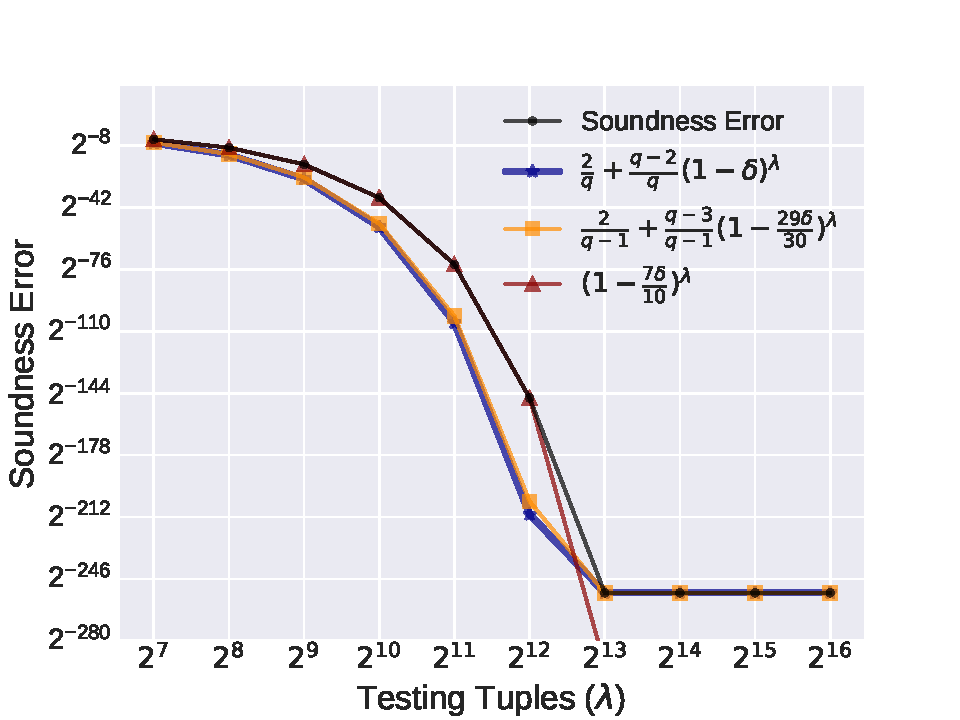
\includegraphics[width=1\textwidth]{graph/se.pdf}
    \caption{Soundness Error of LWE Protocol}
    \label{fig:se}
\end{figure}

Also figure \ref{fig:se} shows the relation between soundness error and the number of testing tuples ($\lambda$). As mentioned in lemma \ref{lemma:lwese}, the soundness error is the maximum value of three individual terms. Figure \ref{fig:se} labels these terms using lines with different colors. When $\lambda$ is small, the soundness error is dominated by $(1 - \frac{7\delta}{10})^\lambda$.
As $\lambda$ increasing, the soundness is decreasing and gradually dominated by $\frac{2}{q-1}$. Hence, the minimum possible soundness is actual independent to the number of testing tuples ($\lambda$), and is determined solely by the field size. In our benchmark, we use a field with size roughly equals to $2^{256}$, therefore, the minimum possible soundness error is around $2^{-256}$.
